\documentclass[conference]{IEEEtran}
\IEEEoverridecommandlockouts
% The preceding line is only needed to identify funding in the first footnote. If that is unneeded, please comment it out.
\usepackage{cite}
\usepackage{amsmath,amssymb,amsfonts}
\usepackage{algorithmic}
\usepackage{algorithm}
\usepackage{graphicx}
\usepackage{textcomp}
\usepackage{xcolor}
\usepackage{tikz}
\usetikzlibrary{shapes.geometric, arrows.meta, positioning}

% Custom Color Definitions for Bar Charts
\definecolor{barAgentic}{RGB}{30, 136, 229}

% ============================================================================
% RESULT PARAMETERS -- the ONLY block to edit when results change (e.g. once
% the zero-day / leave-one-family-out evaluation is finished). Every number
% below is referenced by macro everywhere it appears in the paper (abstract,
% Table II, Results, Conclusion) -- change the value once here and it updates
% everywhere at once. The architecture/methodology sections (III) reference
% no numbers from this block and do not need to change.
%
% NOTE: Fig. 2's per-family precision chart (Section IV-E) uses its own
% literal values in a \foreach list, for TikZ/pgfmath safety -- if these
% change, update that \foreach list too (search "GameHack/91.67").
% ============================================================================
\newcommand{\DatasetTotal}{5,138}   % total graph instances
\newcommand{\TrainCount}{3,596}     % train split size
\newcommand{\ValCount}{513}         % validation split size
\newcommand{\TestCount}{1,029}      % held-out test split size

\newcommand{\MulticlassAcc}{99.61\%}    % 11-class accuracy
\newcommand{\MulticlassMacroF}{99.17\%}     % 11-class macro F1
\newcommand{\MulticlassMacroP}{98.49\%} % 11-class macro precision
\newcommand{\MulticlassMacroR}{99.89\%} % 11-class macro recall

\newcommand{\BinaryAcc}{99.71\%}   % binary accuracy
\newcommand{\BinaryPrec}{99.56\%}  % binary precision
\newcommand{\BinaryRec}{99.78\%}   % binary recall

\newcommand{\AblGnnAcc}{99.32\%}   % ablation: GNN-only accuracy
\newcommand{\AblGnnPrec}{98.47\%}  % ablation: GNN-only precision
\newcommand{\AblGnnRec}{100.0\%}   % ablation: GNN-only recall
\newcommand{\AblPacxAcc}{56.27\%}  % ablation: PAC-X-only accuracy

% Unguarded-retrain repro (scripts/build_retrain_repro.py -> data/retrain_repro/retrain_repro_report.json)
\newcommand{\RetrainPreAcc}{99.61\%}   % before
\newcommand{\RetrainPostAcc}{98.15\%}  % after (best-epoch checkpoint)
\newcommand{\RetrainMidAcc}{87.07\%}   % worst mid-run epoch (epoch 5, early-stopped)

\newcommand{\BenignPrec}{99.83\%}    % per-class: Benign precision
\newcommand{\GandcrabRec}{99.14\%}   % per-class: Gandcrab recall
\newcommand{\GameHackPrec}{91.67\%}  % per-class: GameHack precision (lowest)
\newcommand{\GameHackN}{11}          % per-class: GameHack held-out support
\newcommand{\DarkKometPrec}{95.45\%} % per-class: DarkKomet precision (2nd-lowest)
\newcommand{\DarkKometN}{21}         % per-class: DarkKomet held-out support

% Leave-one-family-out zero-day generalization experiment (scripts/build_zeroday_experiment.py)
\newcommand{\ZDOneFamily}{Emotet}
\newcommand{\ZDOneN}{304}
\newcommand{\ZDOneCatch}{73.68\%}
\newcommand{\ZDOneConf}{68.31\%}
\newcommand{\ZDOneTrigger}{31.58\%}
\newcommand{\ZDTwoFamily}{DarkKomet}
\newcommand{\ZDTwoN}{106}
\newcommand{\ZDTwoCatch}{100\%}
\newcommand{\ZDTwoConf}{99.95\%}
\newcommand{\ZDTwoNearest}{Delf}

% Agent-2 confidence gate: swept against the real fused-confidence pipeline
% (scripts/tune_agent2_threshold.py, data/agent2_tuning/report.json).
\newcommand{\GateTau}{0.68}

% Fail-closed zero-day escalation (scripts/evaluate_zeroday_escalation.py,
% data/agent2_tuning/escalation_report.json). Pooled over all ten
% leave-one-family-out runs: 5,790 benign, 4,050 known-malicious, 2,241 zero-day.
\newcommand{\EscBenignN}{5,790}
\newcommand{\EscKnownMalN}{4,050}
\newcommand{\EscZeroDayN}{2,241}
\newcommand{\EscTotalN}{12,081}
\newcommand{\EscZDBefore}{78.36\%}   % zero-day caught, no escalation
\newcommand{\EscZDAfter}{85.45\%}    % zero-day caught, escalation at tau
\newcommand{\EscKnownBefore}{99.98\%}
\newcommand{\EscKnownAfter}{100.00\%}
\newcommand{\EscFPBefore}{0.57\%}    % benign false positives, no escalation
\newcommand{\EscFPAfter}{3.52\%}     % benign false positives, escalation at tau
\newcommand{\EscCliffTau}{0.72}
\newcommand{\EscCliffFP}{22.49\%}

% Novel-family generalization set: 63 families absent from training, drawn from
% the 7,142-row superset of the source corpus.
\newcommand{\NovelN}{2,004}
\newcommand{\NovelFamilies}{63}
\newcommand{\NovelBefore}{91.37\%}
\newcommand{\NovelAfter}{93.31\%}

% Hard subset: the novel-family samples that actually trip the confidence gate.
\newcommand{\HardN}{56}
\newcommand{\HardBefore}{30.36\%}
\newcommand{\HardAfter}{100\%}

\def\BibTeX{{\rm B\kern-.05em{\sc i\kern-.025em b}\kern-.08em
    T\kern-.1667em\lower.7ex\hbox{E}\kern-.125emX}}
\begin{document}

\title{A Hybrid Graph Attention Network and Heuristic Fusion Framework for Explainable API Threat Detection in Cloud Environments}

\author{\IEEEauthorblockN{Krishna Sowjanya K}
\IEEEauthorblockA{\textit{Department of CSE} \\
\textit{CMR Institute of Technology}\\
Bengaluru, India \\
sowjanya.k@cmrit.ac.in}
\and
\IEEEauthorblockN{Anasuya Chakraborty}
\IEEEauthorblockA{\textit{Department of CSE} \\
\textit{CMR Institute of Technology}\\
Bengaluru, India \\
anch23cs@cmrit.ac.in}
\and
\IEEEauthorblockN{Chandana S}
\IEEEauthorblockA{\textit{Department of CSE} \\
\textit{CMR Institute of Technology}\\
Bengaluru, India \\
chs23cs@cmrit.ac.in}
\and
\IEEEauthorblockN{Dhanyaashri M}
\IEEEauthorblockA{\textit{Department of CSE} \\
\textit{CMR Institute of Technology}\\
Bengaluru, India \\
dhm23cs@cmrit.ac.in}
}

\maketitle

\begin{abstract}
Application Programming Interfaces (APIs) are the primary attack surface for distributed cloud microservices, where obfuscation such as dynamic library hooking and API aliasing lets attackers evade static rule-based heuristics. Cloud API security demands detecting zero-day threats that signatures miss, while deep learning classifiers remain opaque ``black boxes'' unsuited to security operations center (SOC) forensic response. We propose Agentic-PACX, a hybrid framework fusing a Prospect-Aspect-Context (PAC-X) heuristic engine with a structural Graph Attention Network (MalwareGAT) over a 4-node topological graph, arbitrated by a Decision Fusion Layer under two cognitive LLM agents: Agent 1 generates auditable natural-language XAI forensic reports, and Agent 2 gates transfer-learning self-healing on low-confidence detections. On a held-out test set of \TestCount{} real PE-malware graph instances (70/10/20 split, validation-only model selection), MalwareGAT reaches \MulticlassAcc{} accuracy and \MulticlassMacroF{} macro F1 across 11 families, and \BinaryAcc{}/\BinaryPrec{}/\BinaryRec{} accuracy, precision and recall on binary detection. An ablation shows the Fusion Layer safely defers to the structural pathway on this dataset's tabular modality -- its value is arbitration, not a numeric lift. A leave-one-family-out experiment confirms the malicious/benign boundary generalizes to unseen families (\ZDOneCatch{}--\ZDTwoCatch{} catch rates). Since an $\arg\max$ over trained classes absorbs a novel family into the nearest one -- usually benign -- we add a fail-closed rule escalating an uncertain benign verdict to \emph{Suspicious}: over \EscTotalN{} pooled predictions this lifts zero-day recall \EscZDBefore{}$\rightarrow$\EscZDAfter{} for \EscFPAfter{} benign false positives.
\end{abstract}

\begin{IEEEkeywords}
API Security, Threat Detection, Graph Attention Network, Large Language Models, Cloud Computing
\end{IEEEkeywords}

\section{Introduction}
Cloud computing infrastructures rely heavily on Application Programming Interfaces (APIs) for communication between distributed microservices, making APIs a primary attack vector for adversaries seeking to exploit cloud resources, exfiltrate data, or disrupt service. Securing these environments requires identifying not only known malicious signatures, but also the behavioral semantics and structural topology of API call sequences in real time.

Existing security systems predominantly rely on static rule-based heuristics or standard machine learning classifiers. Heuristic engines are fast and deterministic but suffer high false-negative rates against obfuscated or zero-day malware; deep learning models often function as black boxes lacking the explainability rapid forensic response needs; and conventional systems treat API requests as isolated flat sequences rather than interconnected graphs, missing the structural relationships inherent in advanced threats. To address these gaps, this paper proposes Agentic-PACX, an explainable hybrid threat intelligence framework fusing a Prospect-Aspect-Context (PAC-X) heuristic engine with a Graph Attention Network (MalwareGAT), evaluating both deterministic rule violations and topological anomalies. A dual-pathway decision fusion layer, orchestrated by cognitive Large Language Model (LLM) agents, provides human-readable forensic reasoning for every detection and autonomously triggers self-healing transfer-learning loops when model confidence drops, adapting to zero-day threats in real time.

\section{Related Work}
Several studies address malware detection via API-call analysis: system API vectorization \cite{b6}, sequence-representation boosting via API2Vec++ \cite{b15}, \cite{b16}, and deep networks over API sequences in API-MalDetect \cite{b18} and hybrid CNN-DNN mechanisms \cite{b17}. In mobile/IoT domains, API calls, permissions, and opcode features are widely used \cite{b8}, \cite{b10}, \cite{b11}, alongside genetic algorithm-optimized networks \cite{b13}. Beyond isolated malware analysis, AI-enhanced API gateways secure microservices \cite{b5}, complemented by malicious-IP identification \cite{b4}, hybrid deep learning for network-level threats \cite{b1}, EDoS-attack defenses in cloud storage \cite{b3}, and federated IoT security \cite{b9}. Adversaries continuously evolve obfuscated malware to evade static and AI-driven detection \cite{b7}, motivating structural approaches such as CNNs with fuzzy hashing for ransomware \cite{b12} and GNNs, via contextual steerable GNNs for node localization \cite{b2} or graph attention for explainable code localization \cite{b14}.

The evolution of Explainable AI (XAI) in cybersecurity motivates our research. A pivotal advancement is the PAC-X framework by M. Saqib \textit{et al.} \cite{b19}: a Conditional Attention Neural Network (CAN-Net) with Contextual Fuzzy Clustering (CFC), delivering multiclass explainability reported to outperform LIME, LEMNA, and SHAP on explainability power. Agentic-PACX builds on this interpretability philosophy but targets cloud environments via a dual-agent architecture: a GAT for structural dependencies and an LLM-driven fusion framework for natural language explanations. Table \ref{tab:limitations} summarizes existing limitations and our enhancements across five representative methodologies.

\begin{table}[htbp]
\caption{Existing Approaches, Their Limitations, and Agentic-PACX Enhancements}
\label{tab:limitations}
\begin{center}
\resizebox{\columnwidth}{!}{%
\begin{tabular}{|p{0.22\linewidth}|p{0.38\linewidth}|p{0.38\linewidth}|}
\hline
\textbf{Approach / Reference} & \textbf{Existing Research / Limitation} & \textbf{Agentic-PACX Enhancement} \\
\hline
\textbf{PAC-X (CAN-Net) \cite{b19}} & A trained neural classifier over flat tabular features; its fuzzy-clustering (CFC) layer can degrade under concept drift from new variants. & Adds structural GAT attention over graph-topological semantics, plus Agent 2 retraining to counter drift. \\
\hline
\textbf{CNN-DNN Hybrid \cite{b17}} & Builds its API graph via static decompilation (Apktool/smali) before embedding, inheriting static analysis's vulnerability to obfuscation. & Computes GAT attention directly over a lightweight 4-node graph at inference, without a decompilation dependency. \\
\hline
\textbf{GA CNN-SENet \cite{b13}} & Its genetic-algorithm hyperparameter search is a batch, offline procedure with no online adaptation mechanism, and generalization to malware families outside its fixed 8-class evaluation set is not reported. & Deploys Agent 2 for autonomous, real-time transfer-learning self-healing upon low-confidence zero-day events, evaluated directly on held-out samples. \\
\hline
\textbf{API2Vec++ \cite{b15}} & Requires per-sample graph construction and random-walk path generation before BERT embedding, adding preprocessing latency. & Uses lightweight 4-node PyG topological graphs achieving high accuracy with minimal inference latency. \\
\hline
\textbf{API-MalDetect \cite{b18}} & Black-box deep learning output with opaque LIME approximations that lack structural context. & Employs Agent 1 (Forensic LLM) to generate natural language XAI reports directly from edge attention weights. \\
\hline
\end{tabular}%
}
\end{center}
\end{table}

\section{Proposed Methodology}

\subsection{Overview and System Architecture}
Agentic-PACX is a hybrid threat intelligence architecture for detecting malicious API telemetry, obfuscated system calls, and zero-day threat patterns in cloud environments. It orchestrates a dual-pathway pipeline -- (1) a rule-based PAC-X Heuristic Engine and (2) a structural Graph Attention Network (MalwareGAT) -- whose outputs are synthesized within a Decision Fusion Layer, while cognitive LLM agents oversee forensic reasoning (Agent 1) and trigger a self-healing transfer-learning loop (Agent 2) on low-confidence zero-day samples.

\begin{figure*}[htbp]
\centering
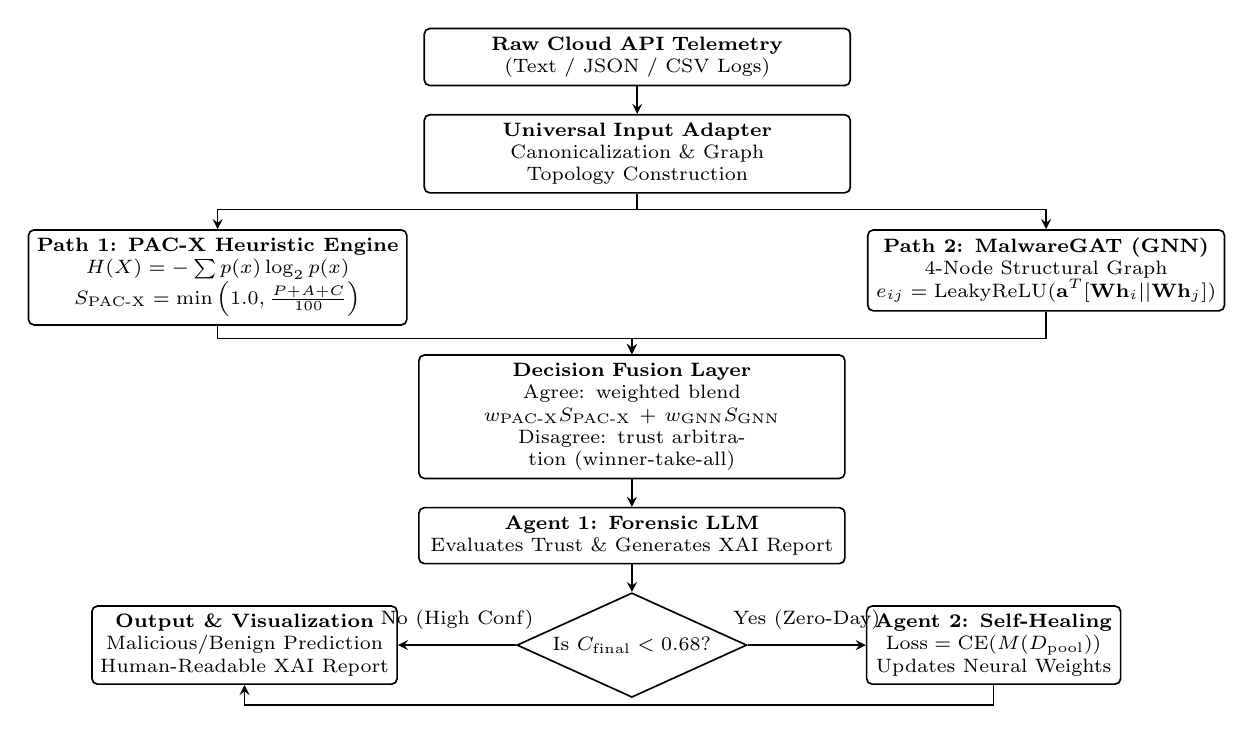
\begin{tikzpicture}[
    node distance=0.35cm and 0.4cm,
    font=\scriptsize,
    base/.style={draw=black, semithick, align=center, fill=white, inner sep=3pt},
    proc/.style={base, rectangle, rounded corners=2pt},
    dia/.style={base, diamond, aspect=2.2, inner sep=2pt},
    arr/.style={->, >=stealth, semithick}
]

% 1. Data Source & Preprocessing
\node[proc, text width=5.2cm] (input) {\textbf{Raw Cloud API Telemetry}\\(Text / JSON / CSV Logs)};

\node[proc, below=0.35cm of input, text width=5.2cm] (adapter) {\textbf{Universal Input Adapter}\\Canonicalization \& Graph Topology Construction};

% 2. Dual Pathways
\node[proc, below left=0.45cm and 0.2cm of adapter] (pacx) {
    \textbf{Path 1: PAC-X Heuristic Engine}\\
    $H(X) = -\sum p(x)\log_2 p(x)$\\
    $S_{\text{PAC-X}} = \min\left(1.0, \frac{P+A+C}{100}\right)$
};

\node[proc, below right=0.45cm and 0.2cm of adapter] (gnn) {
    \textbf{Path 2: MalwareGAT (GNN)}\\
    4-Node Structural Graph\\
    $e_{ij} = \text{LeakyReLU}(\mathbf{a}^T[\mathbf{Wh}_i || \mathbf{Wh}_j])$
};

% 3. Fusion & Agent 1
\path (pacx.south) -- (gnn.south) coordinate[midway] (path_mid);

\node[proc, below=0.45cm of path_mid, text width=5.2cm] (fusion) {
    \textbf{Decision Fusion Layer}\\
    Agree: weighted blend $w_{\text{PAC-X}} S_{\text{PAC-X}} + w_{\text{GNN}} S_{\text{GNN}}$\\
    Disagree: trust arbitration (winner-take-all)
};

\node[proc, below=0.35cm of fusion, text width=5.2cm] (agent1) {
    \textbf{Agent 1: Forensic LLM}\\
    Evaluates Trust \& Generates XAI Report
};

% 4. Condition & Agent 2 / Output
\node[dia, below=0.35cm of agent1] (cond) {Is $C_{\text{final}} < \GateTau$?};

\node[proc, left=1.5cm of cond] (out) {
    \textbf{Output \& Visualization}\\
    Malicious/Benign Prediction\\
    Human-Readable XAI Report
};

\node[proc, right=1.5cm of cond] (agent2) {
    \textbf{Agent 2: Self-Healing}\\
    $\text{Loss} = \text{CE}(M(D_{\text{pool}}))$\\
    Updates Neural Weights
};

% Connections / Arrows
\draw[arr] (input) -- (adapter);
\draw[arr] (adapter.south) -- ++(0,-0.2) -| (pacx.north);
\draw[arr] (adapter.south) -- ++(0,-0.2) -| (gnn.north);

\draw[arr] (pacx.south) |- ([yshift=0.2cm]fusion.north) -- (fusion.north);
\draw[arr] (gnn.south) |- ([yshift=0.2cm]fusion.north) -- (fusion.north);

\draw[arr] (fusion) -- (agent1);
\draw[arr] (agent1) -- (cond);

\draw[arr] (cond.west) -- node[above=2pt, font=\scriptsize, midway] {No (High Conf)} (out.east);
\draw[arr] (cond.east) -- node[above=2pt, font=\scriptsize, midway] {Yes (Zero-Day)} (agent2.west);

\draw[arr] (agent2.south) -- ++(0,-0.25) -| (out.south);

\end{tikzpicture}
\caption{Architectural block diagram of the Agentic-PACX dual-pathway threat detection and self-healing framework.}
\label{fig:architecture}
\end{figure*}

\subsection{Universal Input Adapter and PAC-X Heuristic}

\subsubsection{Input Parsing and Canonicalization}
Cloud API telemetry exhibits structural heterogeneity. The Universal Input Adapter dynamically standardizes arbitrary incoming payloads into a unified PyG graph representation $\mathcal{G} = (\mathcal{V}, \mathcal{E}, \mathbf{X})$. For \emph{raw, unstructured} telemetry (free-text API/behavior logs, or JSON/CSV records not already matching this system's own training schema), the adapter canonicalizes each string token $s$ (lower-cased) in three stages: $\text{LibRef}$ strips a library prefix before ``\texttt{!}''; $\text{SysNorm}$ strips an ``Nt''/``Zw'' kernel-wrapper prefix, guarded to genuine Hungarian-notation casing so it does not fire on a plain module name like \texttt{ntdll}; and $\text{ABISuffix}$ strips an ``A''/``W''/``Ex'' suffix when $|s|>4$ and $s$ is not one of a small set of common unsuffixed names (e.g. \texttt{ShowWindow}):
\begin{equation}
\begin{aligned}
\text{LibRef}(s) &= \begin{cases} \text{substring of } s \text{ after its last "!"} & \text{if "!"} \in s \\ s & \text{otherwise} \end{cases} \\
\text{SysNorm}(s) &= \begin{cases} s[2:] & \text{if } s \text{ starts with "nt"/"zw" (guarded)} \\ s & \text{otherwise} \end{cases} \\
\text{ABISuffix}(s) &= \begin{cases} s[:-1] & |s|{>}4,\ s \text{ ends "a"/"w" (guarded)} \\ s[:-2] & |s|{>}4,\ s \text{ ends "ex"} \\ s & \text{otherwise} \end{cases}
\end{aligned}
\end{equation}
with $\hat{s} = \text{ABISuffix}(\text{SysNorm}(\text{LibRef}(s)))$. This canonicalization, and the MD5 hashing in Eq.~2, is the adapter's deliberately approximate bridge from unstructured logs into the model's 4-node space, since free text cannot supply the structured fields the model was trained on (Section III-B.2).

\subsubsection{Topological Graph Construction}
The adapter extracts feature attributes into semantic node partitions $\mathcal{V} = \{v_0, v_1, v_2, v_3\}$: Node $0$ (PE Header Array $v_0$), Node $1$ (Section Entropy $v_1$), Node $2$ (API Import/Export $v_2$), and Node $3$ (Network Topology $v_3$).

For unstructured string tokens extracted from raw text/API logs -- the case Eq.~1's canonicalization targets -- features are projected into a uniform $256$-dimensional vector space via MD5 bucket hashing:
\begin{equation}
\text{bucket}(s) = \text{MD5}(\hat{s}) \pmod{256}, \quad \hat{\mathbf{u}} = \frac{\mathbf{u}}{\|\mathbf{u}\|_2 + 10^{-8}}
\end{equation}
where $s$ denotes an arbitrary string token, $\hat{s}$ represents its canonicalized form, $\mathbf{u}$ is the raw feature frequency accumulator vector, and $\hat{\mathbf{u}}$ is the resulting L2-normalized vector.

The dataset used to \emph{train} MalwareGAT (Section IV-A) is not raw text: it is a structured static-analysis feature table (PE header fields, section-entropy statistics, and pre-computed continuous embeddings of each sample's import/export lists and string artifacts). All four nodes are therefore built the same way -- each node's numeric column group is projected through the padding/local-standardization operator of Eq.~3, \emph{not} the string-hashing operator of Eq.~2, which is reserved for genuinely unstructured raw-text input. The live Universal Input Adapter reconstructs the identical four vectors whenever an uploaded record matches this native schema, falling back to the Eq.~1--2 hashing bridge otherwise.

\subsubsection{Feature Normalization Formulation}
Each node's feature block is normalized using the static mean $\mu_{i, j}$ and standard deviation $\sigma_{i, j}$ pre-computed across the training split $\mathcal{D}_{\text{train}}$ only (Section IV-A) -- never the validation or test split -- where $\epsilon = 10^{-8}$ prevents division by zero:
\begin{equation}
\mathbf{z}_{i, j} = \frac{\mathbf{x}_{i, j} - \mu_{i, j}}{\sigma_{i, j} + \epsilon}, \quad \forall i \in \{0, \dots, 3\}
\end{equation}
where $\mathbf{x}_{i, j}$ is the raw scalar feature at node $i$, index $j$. These statistics are persisted once and reused identically by the live adapter, so inference is normalized against the same reference distribution used in training.

\subsubsection{PAC-X Heuristic Engine}
Operating in parallel with the GNN, the heuristic engine computes independent signals across three dimensions (Prospect, Aspect, Context). Shannon entropy $H(X)$ is computed for the Prospect score, while Aspect and Context evaluate dangerous APIs and suspicious execution paths:
\begin{equation}
S_{\text{PAC-X}} = \min\left(1.0, \, \frac{S_{\text{prosp}} + S_{\text{aspect}} + S_{\text{context}}}{100.0}\right)
\end{equation}
where $S_{\text{prosp}}$, $S_{\text{aspect}}$, and $S_{\text{context}}$ are sub-scores for payload entropy, suspicious API hooks, and command-line execution contexts. Since these heuristics have signal only on raw text/API-log content, a low-signal input (e.g. a numeric PE-header row with no alphabetic content) is capped below full confidence rather than reporting a spuriously confident ``Benign'' verdict -- Section IV-C's ablation isolates exactly this behavior.

\subsection{MalwareGAT Attention Mechanism}
The graph used by MalwareGAT is represented as $G=(V,E)$. For a node $i$ and neighboring node $j$, the GAT attention score is calculated as:
\begin{equation}
e_{ij} = \mathrm{LeakyReLU} \left( \mathbf{a}^{T} [ \mathbf{W}\mathbf{h}_i \Vert \mathbf{W}\mathbf{h}_j ] \right)
\end{equation}
where $\mathbf{h}_i$ and $\mathbf{h}_j$ are the feature representations of nodes $i$ and $j$, $\mathbf{W}$ is a linear weight projection matrix, $\mathbf{a}$ is the learnable attention vector, and $\Vert$ denotes vector concatenation. The attention scores are normalized using Softmax:
\begin{equation}
\alpha_{ij} = \frac{\exp(e_{ij})}{\sum_{k \in N(i)} \exp(e_{ik})}
\end{equation}
\begin{equation}
\mathbf{h}'_i = \sigma \left( \sum_{j \in N(i)} \alpha_{ij}\mathbf{W}\mathbf{h}_j \right)
\end{equation}
where $N(i)$ represents the 1-hop topological neighborhood of node $i$, $\alpha_{ij}$ is the attention coefficient, and $\sigma(\cdot)$ is the non-linear ELU activation function.

MalwareGAT stacks three GATConv layers, 64 hidden channels per head: 4 heads with concatenation (256-dim) in layer 1, 2 heads concatenated (128-dim) in layer 2, and 1 head, no concatenation (64-dim), in layer 3, each followed by batch normalization and 0.25 dropout. Global mean pooling $\mathbf{h}_{G} = \frac{1}{|V|} \sum_{i \in V}\mathbf{h}'_i$ then feeds a linear classifier. Algorithm \ref{alg:gat} details the forward pass and attention weighting.

\begin{algorithm}[htbp]
\caption{MalwareGAT Forward Pass \& Attention Computation}
\label{alg:gat}
\begin{algorithmic}[1]
\REQUIRE Graph $\mathcal{G} = (\mathcal{V}, \mathcal{E}, \mathbf{X})$, Projection $\mathbf{W}^{(l)}$, Attention $\mathbf{a}^{(l)}$, per-layer heads $K^{(l)} \in \{4, 2, 1\}$ for $l \in \{1, 2, 3\}$.
\ENSURE Graph embedding $\mathbf{h}_G$, Softmax distribution $\hat{\mathbf{y}}_{\text{GNN}}$.
\FOR{each layer $l = 1$ \TO $3$}
    \FOR{each node $i \in \mathcal{V}$}
        \FOR{each attention head $k = 1$ \TO $K^{(l)}$}
            \FOR{each neighbor $j \in \mathcal{N}(i)$}
                \STATE $e_{ij}^{(k)} \leftarrow \text{LeakyReLU}\Big({\mathbf{a}^{(k)}}^\top \big[\mathbf{W}^{(k)}\mathbf{h}_i^{(l-1)} \,\Vert\,$
                \STATE \qquad\qquad\qquad\qquad\quad $\mathbf{W}^{(k)}\mathbf{h}_j^{(l-1)}\big]\Big)$
            \ENDFOR
            \STATE $\alpha_{ij}^{(k)} \leftarrow \frac{\exp(e_{ij}^{(k)})}{\sum_{m \in \mathcal{N}(i)} \exp(e_{im}^{(k)})}$
        \ENDFOR
        \IF{$l < 3$}
            \STATE $\mathbf{h}_i^{(l)} \leftarrow \sigma \left( \Big\Vert_{k=1}^{K^{(l)}} \sum_{j \in \mathcal{N}(i)} \alpha_{ij}^{(k)} \mathbf{W}^{(k)} \mathbf{h}_j^{(l-1)} \right)$ \quad // concat heads
        \ELSE
            \STATE $\mathbf{h}_i^{(l)} \leftarrow \sigma \left( \sum_{j \in \mathcal{N}(i)} \alpha_{ij}^{(1)} \mathbf{W}^{(1)} \mathbf{h}_j^{(l-1)} \right)$ \quad // single head
        \ENDIF
    \ENDFOR
\ENDFOR
\STATE $\mathbf{h}_G \leftarrow \frac{1}{|\mathcal{V}|} \sum_{i \in \mathcal{V}} \mathbf{h}_i^{(3)}$ \quad // Global Mean Pooling
\STATE $\hat{\mathbf{y}}_{\text{GNN}} \leftarrow \text{Softmax}(\mathbf{W}_{\text{out}} \mathbf{h}_G + \mathbf{b}_{\text{out}})$
\RETURN $\mathbf{h}_G, \hat{\mathbf{y}}_{\text{GNN}}$
\end{algorithmic}
\end{algorithm}

\subsection{Decision Fusion Layer and LLM Agents}

\subsubsection{Dynamic Decision Fusion}
The Fusion Layer synthesizes $S_{\text{PAC-X}}$ with the GNN inference score $S_{\text{GNN}}$. Fusion weights adapt dynamically based on Graph Completeness ($C_{\text{graph}}$) and Model Certainty ($\Psi_{\text{certainty}}$):
\begin{equation}
\begin{aligned}
C_{\text{graph}} &= \frac{1}{4}\sum_{i=0}^3 \mathbb{I}(\|\mathbf{x}_i\|_2 > 0) \\
\Psi_{\text{certainty}} &= \text{clamp}\left(0.60 p_1 + 0.40 (p_1 - p_2), 0, 1\right)
\end{aligned}
\end{equation}
where $\mathbb{I}(\cdot)$ is the binary indicator function, and $p_1, p_2$ are the top-2 class probabilities from the GNN output.

Pathway weights start from a 0.6/0.4 GNN/PAC-X baseline, nudged by completeness and certainty ($w_{\text{PAC-X}} = 1 - w_{\text{GNN}}$). On agreement, the fused probability is their weighted blend; on disagreement, the layer arbitrates per-sample by trust instead of averaging the disagreement away:
\begin{equation}
\label{eq:fusion}
\begin{aligned}
w_{\text{GNN}} &= \text{clamp}\big(0.6 {+} 0.2(0.5 C_{\text{graph}} {+} 0.5 \Psi_{\text{certainty}}), 0.5, 0.8\big) \\
S_{\text{fused}} &=
\begin{cases}
w_{\text{PAC-X}} S_{\text{PAC-X}} + w_{\text{GNN}} S_{\text{GNN}} & \text{agree} \\
S_m,\ m = \operatorname*{arg\,max}\limits_{m \in \{\text{PAC-X}, \text{GNN}\}} \text{Trust}_m & \text{disagree}
\end{cases}
\end{aligned}
\end{equation}

\subsubsection{Fail-Closed Zero-Day Escalation}
\label{sec:failclosed}
The fused label is an $\arg\max$ over families the network was \emph{trained} on, so a novel family cannot be named: it is absorbed by the nearest known class, and because the benign cluster is the largest and least structurally distinctive, that class is overwhelmingly ``benign''. A zero-day is by definition an attack, so this is the dangerous failure direction. The pipeline is not oblivious here -- these samples already carry fused confidence below the Agent 2 gate $\tau$ -- but a hard $\arg\max$ discards that signal. We instead reuse it as a decision rule, giving a third verdict state:
\begin{equation}
\label{eq:failclosed}
\hat{y}_{\text{final}} =
\begin{cases}
\text{Suspicious} & \hat{y} = \text{Benign} \ \wedge\ C_{\text{final}} < \tau \\
\hat{y} & \text{otherwise}
\end{cases}
\end{equation}
where $\tau = \GateTau$ (Section~\ref{sec:agent2}). Only a \emph{benign} verdict escalates, since a low-confidence \emph{malicious} one is already actioned; the state is ``Suspicious'' rather than ``Malicious'' because the system has failed to \emph{clear} the sample, not identified an attack; and as a labelling policy over the existing pipeline it changes no weights, so it cannot regress the model. This composes the reject-option formulation \cite{b20} with the fail-closed principle standard in security: abstention resolves toward denial.

\subsubsection{Model Trust Scores (Agent 1)}
When models produce conflicting outputs, Agent 1 assesses relative model trust using multi-term evidential scoring:
\begin{equation}
\begin{aligned}
\text{Trust}_{\text{PAC-X}} &= 0.70 \, \text{Conf}_{\text{PAC-X}} + 0.30 \, E_{\text{PAC-X}} \\
\text{Trust}_{\text{GNN}} &= 0.35 \, p_{\text{raw}} + 0.10 \, \text{Acc} + 0.15 \, C_{\text{graph}} \\
&\quad + 0.25 \, E_{\text{GNN}} + 0.15 \, p_{\text{fam}}
\end{aligned}
\end{equation}
where $E_{\text{PAC-X}}$ and $E_{\text{GNN}}$ denote empirical evidence scores derived from detected API frequencies and attention magnitudes, $p_{\text{fam}}$ represents family classification confidence, and $\text{Acc}$ is the deployed model's own measured overall test accuracy (Section IV-A) -- a fixed, per-model-version prior distinct from $p_{\text{raw}}$'s per-sample confidence, already weighted at 0.35. Agent 1 primes an LLM with the attention matrix $\boldsymbol{\alpha}_{ij}$ to produce XAI reports.

\subsubsection{Autonomous Retraining (Agent 2)}
\label{sec:agent2}
If fused confidence falls below $\tau = \GateTau$, Agent 2 pools the sample for an active transfer-learning self-healing routine (Algorithm \ref{alg:agent2}). The gate is not a round-number default: swept against the true fused-confidence pipeline across all ten leave-one-family-out runs, it captures \EscZDAfter{} of zero-day samples at $\tau = \GateTau$, while beyond $\tau = \EscCliffTau$ false positives rise sharply for diminishing gains -- so $\GateTau$ sits just below that cliff. The same $\tau$ governs the fail-closed rule of Section~\ref{sec:failclosed}, so one threshold carries one meaning: ``the system cannot vouch for this sample.''

\begin{algorithm}[htbp]
\caption{Zero-Day Self-Healing Transfer Learning (Agent 2)}
\label{alg:agent2}
\begin{algorithmic}[1]
\REQUIRE Graph $G$, Confidence $C_{\text{final}}$, Predicted $y_{\text{pred}}$
\ENSURE Updated neural model $M_{\text{live}}$
\IF{$C_{\text{final}} < \GateTau$}
    \STATE $y_{\text{pseudo}} \leftarrow (\hat{y}_{\text{base}} == \text{"Benign"}) \,?\, \text{Class("benign")} : y_{\text{pred}}$
    \STATE $G.y \leftarrow y_{\text{pseudo}}$; \ \ $G.\text{provisional} \leftarrow \text{true}$
    \STATE Ingest $G$ into Retrain Pool $D_{\text{pool}}$
\ENDIF
\STATE \textbf{await} explicit operator trigger \quad // never fires automatically
\STATE $f_{\max} \leftarrow \max_c |\{g \in D_{\text{pool}} : g.y {=} c\}| \,/\, |D_{\text{pool}}|$
\IF{$|\text{classes}(D_{\text{pool}})| < 2$ \OR $f_{\max} > 0.90$}
    \STATE \textbf{refuse} \quad // pool collapsed onto one pseudo-label
\ENDIF
\STATE $M.\text{LoadStateDict}(W_{\text{path}})$
\STATE $\text{Acc}_{\text{pre}} \leftarrow \text{Evaluate}(M, D_{\text{test}})$ \quad // real held-out test set
\FOR{$\text{epoch} = 1$ \TO $10$}
    \STATE $loss \leftarrow \text{CrossEntropyLoss}(M(D_{\text{pool}}))$
    \STATE $loss.\text{Backward}()$; $\text{Opt.Step}()$
\ENDFOR
\STATE $\text{Acc}_{\text{post}} \leftarrow \text{Evaluate}(M, D_{\text{test}})$
\IF{$\text{Acc}_{\text{post}} < \text{Acc}_{\text{pre}} - 0.03$}
    \STATE \textbf{abort} \quad // discard update, keep prior weights
\ELSE
    \STATE $\text{Save}(M.\text{StateDict}(), W_{\text{path}})$
\ENDIF
\RETURN $M_{\text{live}}$
\end{algorithmic}
\end{algorithm}

\section{Results and Discussion}

\subsection{Dataset and Experimental Setup}
The framework was evaluated on a project-derived PE malware dataset of \DatasetTotal{} graph instances across 11 classes: Benign and 10 named malware families from public threat-intelligence feeds (Gandcrab, Emotet, Gamarue, Hotbar, DarkKomet, Delf, Domaiq, DLHelper, DriverPack, GameHack). Four feature groups feed the graph: (1) PE Header structures ($v_0$), (2) section-entropy and structural summary statistics ($v_1$), (3) pre-computed continuous embeddings of each sample's import/export lists ($v_2$), and (4) embeddings of network/string artifacts ($v_3$) -- Section III-B.2 details why all four are real numeric feature blocks, not hashed string tokens. Each node is a 260-dimensional feature vector.

The dataset was partitioned using a 70/10/20 stratified train/validation/test split (seeded per-class for reproducibility): \TrainCount{} training, \ValCount{} validation, and \TestCount{} held-out test samples. The validation split -- not the test split -- drives early stopping and best-checkpoint selection, so the test split is touched exactly once, after model selection is complete, avoiding the optimistic bias of selecting a checkpoint on the same set its final number is reported against.

The system was implemented in PyTorch and PyTorch Geometric (architecture detailed in Section III-C). Optimization uses AdamW with a learning rate of $0.001$ and a weight decay of $1\times 10^{-4}$.

\subsection{Performance Metrics}
Standard metrics are used throughout: Accuracy $= \frac{TP+TN}{TP+TN+FP+FN}$, Precision $= \frac{TP}{TP+FP}$, Recall $= \frac{TP}{TP+FN}$ ($TP, TN, FP, FN$: True/False Positives/Negatives). For class imbalance across the 11 families, unweighted macro-average F1 is used:
\begin{equation}
\text{F1}_{\text{macro}} = \frac{1}{N_c} \sum_{c=1}^{N_c} 2 \times \frac{\text{Prec}_c \times \text{Rec}_c}{\text{Prec}_c + \text{Rec}_c}
\end{equation}
where $N_c = 11$ and $\text{Prec}_c, \text{Rec}_c$ are class-specific metrics.

\subsection{Comparison with Baseline Methods}
Agentic-PACX is compared against five baseline methodologies from recent literature: (1) PAC-X (CAN-Net) \cite{b19}, (2) GA CNN-SENet \cite{b13}, (3) CNN-DNN Hybrid \cite{b17}, (4) API2Vec++ \cite{b15}, and (5) API-MalDetect \cite{b18}. Baseline figures are each paper's own best reported result on its own dataset (Table~\ref{tab:comparison} notes), not a controlled re-evaluation on a shared test set. The Agentic-PACX row reports binary detection on the \TestCount{}-sample held-out test set; multiclass family attribution is in Section IV-E.

\begin{table}[htbp]
\caption{Performance and Explainability Comparison}
\label{tab:comparison}
\begin{center}
\resizebox{\columnwidth}{!}{%
\begin{tabular}{|l|c|c|c|l|}
\hline
\textbf{Methodology} & \textbf{Prec.} & \textbf{Recall} & \textbf{Acc.} & \textbf{Explainability Paradigm} \\
\hline
PAC-X (CAN-Net) \cite{b19}\textsuperscript{a} & 99.77\% & 99.77\% & 99.83\% & Neural + Fuzzy Clustering \\
\hline
GA CNN-SENet \cite{b13}\textsuperscript{b} & 96.19\% & 94.74\% & 92.32\% & Channel Squeeze Weights \\
\hline
CNN-DNN Hybrid \cite{b17}\textsuperscript{c} & N/R & 89.63\% & 96.80\% & Static Feature Weights \\
\hline
API2Vec++ \cite{b15}\textsuperscript{d} & 98.4\% & 95.9\% & 97.3\% & Path-level Walk \\
\hline
API-MalDetect \cite{b18}\textsuperscript{e} & 90.4\% & 98.5\% & 98.8\% & Local LIME Weights \\
\hline
\textbf{Agentic-PACX} & \textbf{\BinaryPrec} & \textbf{\BinaryRec} & \textbf{\BinaryAcc} & \textbf{LLM Agent XAI + Retrain} \\
\hline
\end{tabular}%
}
\end{center}
\footnotesize
\textsuperscript{a}PE-malware result, Table IV of \cite{b19}. \textsuperscript{b}``Total'' row across classes. \textsuperscript{c}Android/APK domain; recall/accuracy are \cite{b17}'s Table II, $K{=}7$ row (its matched pair); Table II omits Precision (N/R). \textsuperscript{d}Classification-task result. \textsuperscript{e}Testset1, $n=100$, malware-class figures.
\end{table}

Agentic-PACX achieves \BinaryAcc{} binary detection accuracy with a lightweight 4-node PyG graph, without API2Vec++'s per-sample random-walk generation or API-MalDetect's LIME post-hoc step -- second only to PAC-X's own 99.83\% figure (a different dataset/protocol). Its differentiating contribution remains lightweight inference plus autonomous LLM forensic reasoning and real-time self-healing retraining, which non-agentic baselines lack.

To honestly evaluate the Decision Fusion Layer's contribution rather than assume it, we ran an ablation isolating each pathway on the same held-out set: GNN-only reaches \AblGnnAcc{} accuracy (\AblGnnPrec{} prec., \AblGnnRec{} recall), while PAC-X evaluated on this dataset's PE-header CSV serialization -- its weaker modality, since no raw text/API-log input exists here -- collapses to predicting the majority (Benign) class on all \TestCount{} samples, \AblPacxAcc{} accuracy with 0\% precision/recall on the malicious class. The fused output matches GNN-only exactly, element-for-element: on disagreement the layer arbitrates by trust score (Eq.~\ref{eq:fusion}), and PAC-X's evidence score collapses to near-zero when guessing Benign on unfamiliar tabular input, so the GNN wins essentially every disagreement. This is an honest, not a null, result -- the fusion layer's contribution here is safe arbitration, not a numeric accuracy lift; PAC-X's designed value is expected to materialize on its intended raw API-log/text modality instead. (The \AblGnnAcc{} GNN-only figure reflects the deployed live-inference pathway, which blends the raw softmax with a class-centroid similarity and evidence term; the plain-argmax figure in Table~\ref{tab:comparison}, \BinaryAcc{}, is marginally higher.)

\subsection{Explainability and Zero-Day Adaptation}
A major advantage of MalwareGAT is its ability to expose learned attention weights $\alpha_{ij}$ associated with graph edges, indicating relative importance during message passing. Agent 1 ingests these topological weights to generate natural language forensic explanations, such as the following representative example:

\begin{quote}
\textit{``Agent 1 Forensic Rationale: Critical structural anomaly detected between Node 0 (PE Header) and Node 2 (API Export) with an attention weight of 0.89. Indicates obfuscated CreateRemoteThread injection into dynamic cloud endpoints.''}
\end{quote}

Agent 2 pools low-confidence observations ($C_{\text{final}} < \GateTau$) for a 10-epoch transfer-learning loop (Algorithm~\ref{alg:agent2}), bounded by two guardrails: a pool collapsed onto one pseudo-label is refused, and a post-fine-tune check discards the update if held-out accuracy regresses by more than 3 points. Both follow from a controlled reproduction: an unguarded retrain on a tiny single-class pool regressed held-out accuracy from \RetrainPreAcc{} to \RetrainPostAcc{} even with best-epoch selection, and to \RetrainMidAcc{} mid-run -- direct evidence of the catastrophic forgetting they prevent.

The evaluations above measure accuracy on \emph{known} families seen during training. To directly test generalization to a genuinely unseen threat, we ran a leave-one-family-out experiment: retraining MalwareGAT from scratch with one family excluded entirely from train/validation/test, then evaluating only on that family's untouched samples. Holding out \ZDOneFamily{} (\ZDOneN{} samples) yielded a \ZDOneCatch{} zero-day catch rate (flagged malicious, not benign) at \ZDOneConf{} mean confidence, with \ZDOneTrigger{} of samples correctly triggering Agent 2's low-confidence pathway; holding out \ZDTwoFamily{} (\ZDTwoN{} samples) yielded a \ZDTwoCatch{} catch rate at \ZDTwoConf{} confidence, confidently but incorrectly attributed to \ZDTwoNearest{}, its nearest known family, rather than flagged as uncertain. Together these show the malicious/benign boundary generalizes past the training classes -- via similarity to the nearest known malicious cluster rather than a dedicated novelty detector -- and that Agent 2's confidence gate engages precisely when that generalization is uncertain rather than confidently wrong.

Pooling all ten held-out runs (\EscTotalN{} predictions: \EscBenignN{} benign, \EscKnownMalN{} known-malicious, \EscZeroDayN{} zero-day) through the deployed fusion pipeline, the residual errors are almost entirely novel malware labelled \emph{benign}. Applying (\ref{eq:failclosed}) at $\tau = \GateTau$ raises zero-day recall \EscZDBefore{}$\rightarrow$\EscZDAfter{} and known-malware detection \EscKnownBefore{}$\rightarrow$\EscKnownAfter{}, for \EscFPAfter{} benign false positives (from \EscFPBefore{}) -- about one benign sample in twenty-eight withheld rather than cleared. The gain concentrates where it should: across \NovelN{} samples from \NovelFamilies{} unseen families recall moves only \NovelBefore{}$\rightarrow$\NovelAfter{}, most already being confidently flagged, but on the \HardN{}-sample subset whose confidence actually trips the gate it rises \HardBefore{}$\rightarrow$\HardAfter{} -- the gate had flagged all \HardN{} while the label cleared 39, so the evidence was present and merely unused. Beyond $\tau = \EscCliffTau$ false positives jump to \EscCliffFP{}, the practical ceiling; since escalation relabels after fusion and trains nothing, accuracies reported elsewhere are unaffected.

\subsection{Multi-Class Threat Family Evaluation}
To evaluate fine-grained threat discrimination beyond binary classification, the MalwareGAT neural stack was evaluated across the 11 real classes present in the dataset (Benign, Gandcrab, Emotet, Gamarue, Hotbar, DarkKomet, Delf, Domaiq, DLHelper, DriverPack, and GameHack), achieving \MulticlassAcc{} overall accuracy and a \MulticlassMacroF{} macro F1-score (\MulticlassMacroP{} macro precision, \MulticlassMacroR{} macro recall) on the \TestCount{}-sample held-out test set. Precision was consistently high across every family: 100\% on seven of eleven (Delf, Domaiq, DLHelper, DriverPack, Emotet, Gamarue, Gandcrab -- the last at \GandcrabRec{} recall), and \BenignPrec{} on Benign. The lowest precision was on GameHack (\GameHackPrec{}, \GameHackN{} samples) and DarkKomet (\DarkKometPrec{}, \DarkKometN{} samples) -- both among the smallest-support families, consistent with the natural difficulty of estimating precision from few held-out examples rather than a systematic weakness. Fig.~\ref{fig:perfamily} shows per-family precision, mirroring the live per-family metrics chart in the deployed system.

\begin{figure}[htbp]
\centering
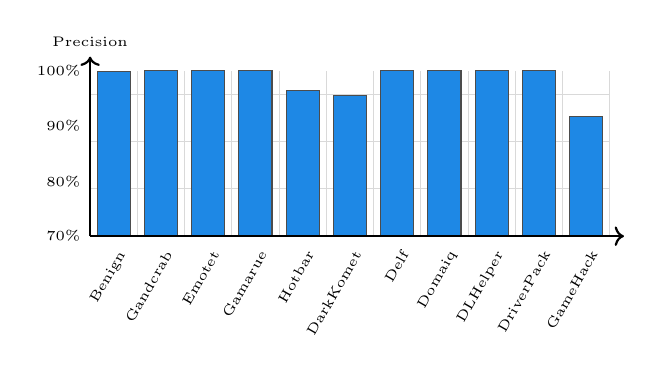
\begin{tikzpicture}[font=\tiny, scale=0.6]
    \draw[gray!30, thin] (0,0) grid (11,3.5);
    \node[left] at (0,0) {70\%};
    \node[left] at (0,1.16) {80\%};
    \node[left] at (0,2.33) {90\%};
    \node[left] at (0,3.5) {100\%};
    \foreach \x/\name/\val in {
        0/Benign/99.83, 1/Gandcrab/100.0, 2/Emotet/100.0, 3/Gamarue/100.0,
        4/Hotbar/96.43, 5/DarkKomet/95.45, 6/Delf/100.0, 7/Domaiq/100.0,
        8/DLHelper/100.0, 9/DriverPack/100.0, 10/GameHack/91.67} {
        \pgfmathsetmacro{\ypos}{(\val-70)/30*3.5}
        \draw[fill=barAgentic, draw=black!70] (\x+0.15,0) rectangle (\x+0.85,\ypos);
        \node[below, rotate=60, anchor=north east, font=\tiny] at (\x+0.5,0) {\name};
    }
    \draw[->, thick] (0,0) -- (0,3.8) node[above] {Precision};
    \draw[->, thick] (0,0) -- (11.3,0);
\end{tikzpicture}
\caption{Per-family precision on the \TestCount{}-sample held-out test set.}
\label{fig:perfamily}
\end{figure}

\section{Conclusion and Future Work}
We presented Agentic-PACX, a hybrid threat intelligence framework combining a rule-based Prospect-Aspect-Context (PAC-X) heuristic engine with a structural Graph Attention Network (MalwareGAT), fused under trust-based arbitration and governed by dual cognitive LLM agents. Across \DatasetTotal{} graph instances spanning 11 real-world malware families (\TestCount{} held-out samples, validation-only model selection), it achieved \BinaryAcc{}/\BinaryPrec{}/\BinaryRec{} binary accuracy, precision and recall, and \MulticlassAcc{} accuracy with \MulticlassMacroF{} macro F1 on family attribution. An ablation showed the Decision Fusion Layer safely defers to the structural pathway on this dataset's tabular modality, contributing arbitration and safety rather than an accuracy lift. A leave-one-family-out experiment confirmed generalization to entirely unseen families, with Agent 2's gate engaging where that generalization was uncertain rather than confidently wrong. Where it still failed, the residual errors were overwhelmingly novel malware labelled benign -- an artifact of forcing an $\arg\max$ over trained classes onto a family belonging to none of them. Reusing the gate as a fail-closed rule (Section~\ref{sec:failclosed}) converts that measured uncertainty into a third \emph{Suspicious} verdict, lifting zero-day recall \EscZDBefore{}$\rightarrow$\EscZDAfter{} over \EscTotalN{} predictions -- and \HardBefore{}$\rightarrow$\HardAfter{} on the subset handled worst -- for \EscFPAfter{} false positives, without altering a learned parameter.

Agent 1 bridges the black-box gap by translating edge attention weights into auditable XAI forensic reports; Agent 2 establishes a self-healing loop, guarded by pool-diversity and accuracy-regression checks that a controlled reproduction confirmed prevent a poorly-formed retrain batch from silently degrading a converged model. Two limitations bound these claims: escalation catches only novel malware whose confidence falls below $\tau$, so families placed \emph{confidently} in the wrong class dominate the residual misses -- a representational gap no threshold can close; and Agent 2's pool is pseudo-labelled by the model's own prediction at exactly the moment it is unreliable, so labels are kept provisional and a collapsed pool is refused for retraining. Future work will add open-set novelty detection alongside the gate, replace pseudo-labelling with partial supervision that does not force a wrong family label, deploy on production cloud API gateways to measure latency, validate PAC-X on its native raw-text modality, and expand federated threat-intelligence sharing across multi-cloud edge environments.

\begingroup
\footnotesize
\begin{thebibliography}{00}
\bibitem{b1} M. Premkumar \textit{et al.}, ``Hybrid Deep Learning Model for Cyber-Attack Detection,'' in \textit{ICICCS}, Madurai, India, 2023, pp. 1435--1441.
\bibitem{b2} M. S. Ananth Kumar \textit{et al.}, ``Energy efficient contextual steerable crayfish graph neural network with hybrid binary light spectrum atomic orbital optimization-based node localization and attack detection in WSNs,'' in \textit{Proc. ICMSCE}, 2025.
\bibitem{b3} A. Karthika, N. Muthukumaran, and J. S. Raj, ``An Ads-Csab approach for economic denial of sustainability attacks in cloud storage,'' \textit{Int. J. Sci. \& Technol. Res.}, vol. 9, no. 4, pp. 2962--2967, April 2020.
\bibitem{b4} A. A. Siam \textit{et al.}, ``A Robust Algorithm for Identifying Malicious IPs Enhancing Cybersecurity Defense,'' in \textit{IEEE MPCON}, Jabalpur, India, 2025, pp. 486--492.
\bibitem{b5} K. K. Ratra \textit{et al.}, ``AI-Enhanced API Gateway: A Unified Framework for Security and Performance for Next Generation Microservices,'' in \textit{IEEE IEMCON}, Berkeley, CA, USA, 2025, pp. 0577--0584.
\bibitem{b6} K. Shin \textit{et al.}, ``System API Vectorization for Malware Detection,'' IEEE Access, vol. 11, pp. 53788--53805, 2023.
\bibitem{b7} S. Chandran \textit{et al.}, ``From Static to AI-Driven Detection: A Comprehensive Review of Obfuscated Malware Techniques,'' IEEE Access, vol. 13, pp. 74335--74358, 2025.
\bibitem{b8} A. Srinivasan \textit{et al.}, ``Smarter Cyber Defense: Machine Learning-Based Malicious File Detection,'' in \textit{IEEE AECE}, Ghaziabad, India, 2025, pp. 308--312.
\bibitem{b9} X. Pei \textit{et al.}, ``A Knowledge Transfer-Based Semi-Supervised Federated Learning for IoT Malware Detection,'' IEEE Trans. Dependable Secure Comput., vol. 20, no. 3, pp. 2127--2143, May--June 2023.
\bibitem{b10} A. Museeb \textit{et al.}, ``Android Malware Detection Using API Calls and Permissions With Random Forest Classifier,'' IEEE Access, vol. 14, pp. 6464--6480, 2026.
\bibitem{b11} H. Lee \textit{et al.}, ``Robust IoT Malware Detection and Classification Using Opcode Category Features on Machine Learning,'' IEEE Access, vol. 11, pp. 18855--18867, 2023.
\bibitem{b12} H. Rodriguez-Bazan, G. Sidorov, and P. J. Escamilla-Ambrosio, ``Android Ransomware Analysis Using Convolutional Neural Network and Fuzzy Hashing Features,'' IEEE Access, vol. 11, pp. 121724--121738, 2023.
\bibitem{b13} Z. Yang \textit{et al.}, ``A Malware Detection Method Based on Genetic Algorithm Optimized CNN-SENet Network,'' IEEE Access, vol. 12, pp. 160052--160063, 2024.
\bibitem{b14} M. C. Ipek and S. Sen, ``Explainable android malware detection and malicious code localization using graph attention,'' J. Inf. Secur. Appl., vol. 98, 2026, Art no. 104385.
\bibitem{b15} L. Cui \textit{et al.}, ``API2Vec++: Boosting API Sequence Representation for Malware Detection and Classification,'' IEEE Trans. Softw. Eng., vol. 50, no. 8, pp. 2142--2162, Aug. 2024.
\bibitem{b16} W. Sun, ``Malicious software identification based on deep learning algorithms and API feature extraction,'' EURASIP J. Inf. Secur., vol. 2025, 2025, Art no. 10, doi: 10.1186/s13635-025-00197-4.
\bibitem{b17} S. Dong, L. Shu, and S. Nie, ``Android Malware Detection Method Based on CNN and DNN Hybrid Mechanism,'' IEEE Trans. Ind. Inform., vol. 20, no. 5, pp. 7744--7753, May 2024.
\bibitem{b18} P. Maniriho, A. N. Mahmood, and M. J. M. Chowdhury, ``API-MalDetect: Automated malware detection framework for windows based on API calls and deep learning techniques,'' J. Netw. Comput. Appl., vol. 218, 2023, Art no. 103704.
\bibitem{b19} M. Saqib, B. C. M. Fung, and P. Charland, ``PAC-X: Fuzzy Explainable AI for Multiclass Malware Detection,'' IEEE Trans. Fuzzy Syst., vol. 34, no. 1, pp. 53--64, Jan. 2026.
\bibitem{b20} C. K. Chow, ``On optimum recognition error and reject tradeoff,'' IEEE Trans. Inf. Theory, vol. 16, no. 1, pp. 41--46, Jan. 1970.
\end{thebibliography}
\endgroup

\end{document}
